\documentclass{beamer}\usepackage{graphicx, color}
%% maxwidth is the original width if it is less than linewidth
%% otherwise use linewidth (to make sure the graphics do not exceed the margin)
\makeatletter
\def\maxwidth{ %
  \ifdim\Gin@nat@width>\linewidth
    \linewidth
  \else
    \Gin@nat@width
  \fi
}
\makeatother

\IfFileExists{upquote.sty}{\usepackage{upquote}}{}
\definecolor{fgcolor}{rgb}{0.2, 0.2, 0.2}
\newcommand{\hlnumber}[1]{\textcolor[rgb]{0,0,0}{#1}}%
\newcommand{\hlfunctioncall}[1]{\textcolor[rgb]{0.501960784313725,0,0.329411764705882}{\textbf{#1}}}%
\newcommand{\hlstring}[1]{\textcolor[rgb]{0.6,0.6,1}{#1}}%
\newcommand{\hlkeyword}[1]{\textcolor[rgb]{0,0,0}{\textbf{#1}}}%
\newcommand{\hlargument}[1]{\textcolor[rgb]{0.690196078431373,0.250980392156863,0.0196078431372549}{#1}}%
\newcommand{\hlcomment}[1]{\textcolor[rgb]{0.180392156862745,0.6,0.341176470588235}{#1}}%
\newcommand{\hlroxygencomment}[1]{\textcolor[rgb]{0.43921568627451,0.47843137254902,0.701960784313725}{#1}}%
\newcommand{\hlformalargs}[1]{\textcolor[rgb]{0.690196078431373,0.250980392156863,0.0196078431372549}{#1}}%
\newcommand{\hleqformalargs}[1]{\textcolor[rgb]{0.690196078431373,0.250980392156863,0.0196078431372549}{#1}}%
\newcommand{\hlassignement}[1]{\textcolor[rgb]{0,0,0}{\textbf{#1}}}%
\newcommand{\hlpackage}[1]{\textcolor[rgb]{0.588235294117647,0.709803921568627,0.145098039215686}{#1}}%
\newcommand{\hlslot}[1]{\textit{#1}}%
\newcommand{\hlsymbol}[1]{\textcolor[rgb]{0,0,0}{#1}}%
\newcommand{\hlprompt}[1]{\textcolor[rgb]{0.2,0.2,0.2}{#1}}%

\usepackage{framed}
\makeatletter
\newenvironment{kframe}{%
 \def\at@end@of@kframe{}%
 \ifinner\ifhmode%
  \def\at@end@of@kframe{\end{minipage}}%
  \begin{minipage}{\columnwidth}%
 \fi\fi%
 \def\FrameCommand##1{\hskip\@totalleftmargin \hskip-\fboxsep
 \colorbox{shadecolor}{##1}\hskip-\fboxsep
     % There is no \\@totalrightmargin, so:
     \hskip-\linewidth \hskip-\@totalleftmargin \hskip\columnwidth}%
 \MakeFramed {\advance\hsize-\width
   \@totalleftmargin\z@ \linewidth\hsize
   \@setminipage}}%
 {\par\unskip\endMakeFramed%
 \at@end@of@kframe}
\makeatother

\definecolor{shadecolor}{rgb}{.97, .97, .97}
\definecolor{messagecolor}{rgb}{0, 0, 0}
\definecolor{warningcolor}{rgb}{1, 0, 1}
\definecolor{errorcolor}{rgb}{1, 0, 0}
\newenvironment{knitrout}{}{} % an empty environment to be redefined in TeX

\usepackage{alltt}
\usetheme{Stats}
\setbeamercovered{transparent}
\usepackage{color}
\usepackage{hyperref}
  \hypersetup{
  	colorlinks=true
		linkcolor=black
		}
\usepackage{url}
\usepackage{graphics}
\usepackage{tikz}
\usepackage{booktabs}





%%%%%%%%%%%%%%%%%%%%%%%%%%%%%%%% Title Slide %%%%%%%%%%%%%%%%%%%%%%%%%%
\title[]{Intro to Social Science Data Analysis \\[1cm] Week 12 Lecture: Multivariate Linear Regression \& Presenting Regression Results}
\author[]{
    \href{mailto:gandrud@yonsei.ac.kr}{Christopher Gandrud}
}
\date{\today}


\begin{document}

\frame{\titlepage}

\section[Outline]{}
\frame{\tableofcontents}

%%%%%%%%%% Assignment 3
\section{Assignment 3}
\frame{
  \frametitle{Assignment 3}
  \begin{itemize}
    \item There was an extremely \textbf{bimodal} distribution to the Assignment 3 scores.
    \item We should care about \textbf{learning} rather than \textbf{grades}.
    \item So, if you received below an 80\% I want to work with you to make sure you actual \textbf{learn} the material.
    \item By Friday come to my office with:
    \begin{itemize}
      \item a description of what steps you need to take to complete each question,
      \item identification of where in the lecture slides you can find the code to complete these steps.
    \end{itemize}
    \item Then redo the assignment by next Tuesday (27 November) and you can receive \textbf{up to an 85\% on the assignment}.
  \end{itemize}
}

%%%%%%%%%% Assignment 4
\section{Assignment 4}
\frame{
  \frametitle{Assignment 4}
  Due: Friday 30 November \\[0.5cm]
  {\Large{Research Design}} \\[0.25cm]
  With your partner plan your research by answering the following questions:
  \begin{enumerate}
    \item What difference or anomaly do you want to explain?
    \item What is your best guess explanation? Draw your best guess in a diagram.
    \item Can you test your hypothesis using data? If so, what data do you need to collect and what tests could you use?
    \item What rival explanations are their?
    \item How could you use data to test whether your best guess or the rival explanations are better? Write this as an \textbf{equation} if possible.
    \item What other factors may influence the relationship you observe?
  \end{enumerate}
{\tiny{Questionnaire from: modified from Cheryl Schonhardt-Bailey}}
}

%%%%%%%%%%% Recap
\section{Recap}
\frame{
	\frametitle{Quick Quiz 1}
{\Large{Interpret the following correlations ($R$):}} \\[0.5cm]
  \begin{itemize}
    \item $R = 0.91$
    \item $R = 0.02$
    \item $R = -0.3$
  \end{itemize}
}

\frame{
  \frametitle{Quick Quiz 2}
  What is a residual?\\[0.5cm]
  Discuss at least \textbf{two} things that residuals are used for in simple linear regression?
}

\frame{
  \frametitle{Quick Quiz 3}
  What assumptions does the linear regression model make?
}

\frame{
  \frametitle{Quick Quiz 4}
  Create a hypothesis test for a linear regression coefficient ($\hat{\beta}$)
}

\frame{
  \frametitle{Quick Quiz 5}
  How do you interpret a linear regression coefficient for a dummy variable?
}

%%%%%% Multiple Linear Regression
\section{Multiple Linear Regression}
\frame{
  \frametitle{Intro to Multiple Linear Regression}
  Last class we learned how to use the tools of simple linear regression to examine the \textbf{bivariate} relationship between a dependent variable and \textbf{one independent} variable. \\[0.5cm]
  What if we want to examine \textbf{multivariate relationships}, i.e. the relationship between a dependent variable and \textbf{multiple} independent variables at the same time? \\[0.5cm]
  In these cases we can use \textbf{multiple linear regression}.
}

\frame{
  \frametitle{Why?}
  \begin{center}
{\Large{\textbf{Why} would we want to examine multiple independent variables at the same time?}}
  \end{center}
}

\frame{
  \frametitle{Minimal criteria for making a causal argument}
  To make a \textbf{probabilistic causal argument}, i.e. ``$X$ caused $Y$" we need to meet \emph{at least} three criteria:
  \begin{itemize}
    \item $X$ is \textbf{statistically associated} with $Y$,
    \item $X$ happens before $Y$ (i.e. \textbf{time order}),
    \item all \textbf{alternative explanations} for the association are ruled out.
  \end{itemize}    
}

\frame{
  \frametitle{Time Order \& Causality}
  {\Large{Linear regression per se can't help us establish time order. \\[0.5cm]
  We need to understand our data to do that. \\[0.5cm]
  We may also need to take measurements at multiple points in time and use more advanced statistical tools than the ones covered in this course.}}
}

\frame{
  \frametitle{Simple Linear Regression \& Causality}
{\Large{Simple Linear Regression is a tool we can use to establish the statistical association between $X$ and $Y$. \\[0.5cm]
  How can we determine how much if at all, the value of $Y$ is actually explained by the value of $X$ and not some other alternative factor(s)?}}
}

\frame{
  \frametitle{Spurious Example}
{\Large{A silly example:}} \\[0.5cm]
  You are interested in what causes expensive fire damage. \\[0.25cm]
  You observe that the most expensive fires have the most fire trucks on the scene. \\[0.25cm]
  Did having more fire trucks cause more damage?
}

\frame{
  \frametitle{Spurious Example}
  Clearly, the \emph{size of the fire} caused both the amount of fire damage and the number of fire trucks that responded. \\[0.5cm]
  There is a \textbf{spurious relationship} between number of fire trucks and fire damage.
}

\frame{
  \frametitle{Spurious Diagram}
  \begin{figure}
    \caption{Spurious Relationship}
    \begin{tikzpicture}
      \vspace{0.5cm}
      %% Nodes
      \node (z) at (0,0) {$Z$};
      \node (x) at (-2, 2) {$X$};
      \node (y) at (2, 2) {$Y$};
      
      %% Arrows
      \draw[->] (z) -- (x);
      \draw[->] (z) -- (y);
      
    \end{tikzpicture}
  \end{figure}
}

\frame{
  \frametitle{Controlling for $Z$}
  If we were able to run an experiment where we \textbf{randomized} the units who are given `treatment' $X$ and those that are not (the `control' group). \\[0.5cm]
  On average the units will have the same values of $Z$. \\[0.5cm]
  We can say that we are \bf{controlling for} $Z$. \\[0.5cm]
  If, after randomization, the association between $X$ and $Y$ still exists, then we have found evidence to rule out alternative explanations.
}

\frame{
  \frametitle{Observational Data}
  However, in many social science situations we cannot run an experiment with randomized control and treatment groups. \\[0.5cm]
  For example, we cannot randomly assign people to live in dictatorships and democracies. \\[0.5cm]
  In these cases we need to use \textbf{statistical control} like \bf{multiple linear regression}.
}

\frame{
  \frametitle{Note:}
  In many cases social scientists actually do conduct randomized experiments. \\[0.5cm]
  For example, the Obama campaign randomized the email messages it sent to people asking for donations. \\[0.5cm]
  Also, there are more advanced statistical techniques that can be combined with multiple linear regression to enhance statistical control. For example, matching.
}

\frame{
  \frametitle{Multi-causality}
  Also, in the social sciences something \emph{rarely has one cause}. \\[0.5cm]
  Instead, phenomenon usually have multiple causes; each making a contribution to the probable value of an outcome. \\[0.5cm]
  Multiple linear regression is a statistical tool that we can use to help identify the \textbf{individual} contribution of some factor to an outcome, \textbf{controlling for} other factors.
}

\frame{
  \frametitle{The Multiple Linear Regression Model}
  An estimated multiple linear regression model for predictors $x_{1} \ldots x_{p}$:
  \[
  \hat{y} = \alpha + \beta_{1}x_{1} + \beta_{2}x_{2} + \ldots + \beta_{p}x_{p} 
  \]
}

\begin{frame}[fragile]
  \frametitle{Today's Data}
\begin{knitrout}
\definecolor{shadecolor}{rgb}{0.969, 0.969, 0.969}\color{fgcolor}\begin{kframe}
\begin{alltt}
\hlcomment{# Load library}
\hlfunctioncall{library}(openintro)

\hlcomment{# Load data}
\hlfunctioncall{data}(marioKart)

\hlcomment{# Show Variables}
\hlfunctioncall{names}(marioKart)
\end{alltt}
\begin{verbatim}
##  [1] "ID"         "duration"   "nBids"     
##  [4] "cond"       "startPr"    "shipPr"    
##  [7] "totalPr"    "shipSp"     "sellerRate"
## [10] "stockPhoto" "wheels"     "title"
\end{verbatim}
\end{kframe}
\end{knitrout}

\end{frame}

\frame{
  \frametitle{Example Multiple Linear Regression Model}
  Imagine we are interested in what explains the EBay selling price of the game Mario Kart (\texttt{totalPr})? \\[0.5cm]
  We want to see if the duration of the auction in days (\texttt{duration}), whether the game was in used condition (\texttt{condused}), and the number of wheels included in the auction (\texttt{wheels}) impacted the selling price.
}

\begin{frame}[fragile]
  \frametitle{Scatter}
\begin{knitrout}
\definecolor{shadecolor}{rgb}{0.969, 0.969, 0.969}\color{fgcolor}

{\centering 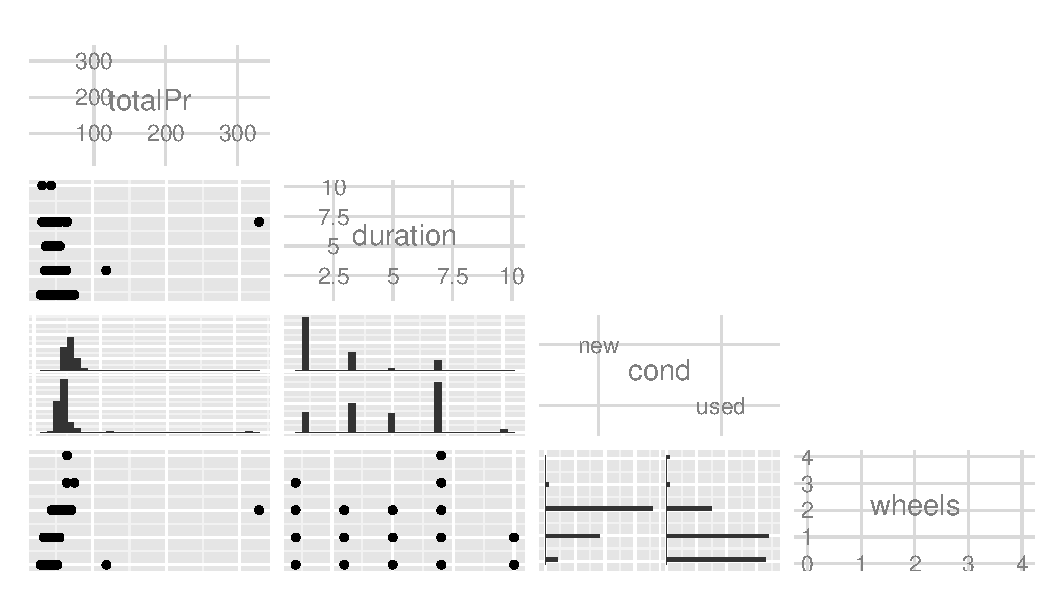
\includegraphics[width=\maxwidth]{figure/Scatter} 

}


\end{knitrout}

\end{frame}

\frame{
  \frametitle{Sum of Squared Residuals}
  Estimating the coefficients and making inferences about them is similar to simple linear regression. \\[0.5cm]
  For example, to find the sum of the squared residuals:
  \[
  SSR = \sum^{n}_{i=1} = e^{2}_{i} = \sum^{n}_{i=1} = (y_{i} + \hat{y}_{i})^{2} 
  \]
}

\begin{frame}[fragile]
  \frametitle{Estimation}
  Estimating the $\beta$s by hand in multiple linear regression is very difficult, but it is relatively easy if you let R do the hard work with the \texttt{lm} command:
\begin{knitrout}
\definecolor{shadecolor}{rgb}{0.969, 0.969, 0.969}\color{fgcolor}\begin{kframe}
\begin{alltt}
\hlcomment{# Estimated multivariate linear regression model}
M1 <- \hlfunctioncall{lm}(totalPr ~ duration + cond + 
           wheels, data = marioKart)
\end{alltt}
\end{kframe}
\end{knitrout}

\end{frame}

\begin{frame}[fragile]
  \frametitle{Showing the Coefficient Estimates}
\begin{knitrout}
\definecolor{shadecolor}{rgb}{0.969, 0.969, 0.969}\color{fgcolor}\begin{kframe}
\begin{alltt}
\hlcomment{# Show coefficient point estimates}
M1
\end{alltt}
\begin{verbatim}
## 
## Call:
## lm(formula = totalPr ~ duration + cond + wheels, data = marioKart)
## 
## Coefficients:
## (Intercept)     duration     condused  
##      35.735        0.680       -0.695  
##      wheels  
##      10.455
\end{verbatim}
\end{kframe}
\end{knitrout}

What is the estimated linear regression equation?
\end{frame}

\frame{
  \frametitle{Linear Regression Equation}
  \[
  \widehat{\tt{totalPr}} = 35.74 + 0.68\tt{duration} + -0.695\tt{condused} + 10.46\tt{wheels}
  \]
}

\frame{
  \frametitle{Question Linear Regression Equation}
  \[
  \begin{split}
  \widehat{\tt{totalPr}} = & \left 35.74 + 0.68(\tt{duration}) + \right. \\
                          & \left -0.695(\tt{condused}) + 10.46(\tt{wheels}) \right)
  \end{split}
  \]
  What do you estimated will be the total selling price for a Mario Kart auction that was 5 days long, was in new condition, and included 2 wheels?
}

\frame{
  \frametitle{Linear Regression Equation Estimated $Y$}
  \[
  60.06 = 35.74 + 0.68(5) + -0.695(0) + 10.46(2)
  \]
}

\frame{
  \frametitle{Single Variable Interpretation}
  We can interpret the effect of \texttt{duration} like this:
  \begin{quote}
    Controlling for the condition of the game and the number of wheels included, each day a Mario Kart EBay auction continues I expect that the total selling price will increase by 0.68.
  \end{quote}
   \hline \vspace{0.5cm}
For the dummy variable \texttt{condused} we have the following interpretation:
\begin{quote}
    Controlling for the duration of the auction and the number of wheels sold, I expect used Mario Kart games to sell for 0.695 less than new games in EBay auctions.
 \end{quote}
}

\frame{
  \frametitle{Remember the Units}
  \begin{center}
{\Large{Remember that the coefficients are in terms of the variables' units. \\[0.5cm]
  A large coefficient does not necessarily mean a big effect.}}
  \end{center}
}

%%% Multinomial variables
\begin{frame}[fragile]
  \frametitle{Multinomial Variables in Multiple Linear Regression}
  \begin{center}
  What if an independent variable has more than two category?
  \end{center}
  For example,  the shipping method variable \texttt{shipSp} has the following categories:
\begin{knitrout}
\definecolor{shadecolor}{rgb}{0.969, 0.969, 0.969}\color{fgcolor}\begin{kframe}
\begin{alltt}
\hlfunctioncall{summary}(marioKart$shipSp)
\end{alltt}
\begin{verbatim}
## firstClass      media      other     parcel 
##         22         14          3         16 
##   priority   standard    ups3Day  upsGround 
##         23         33          1         31
\end{verbatim}
\end{kframe}
\end{knitrout}

\end{frame}

\begin{frame}[fragile]
  \frametitle{Linear Model with Multinomial Independent Variables}
\begin{knitrout}
\definecolor{shadecolor}{rgb}{0.969, 0.969, 0.969}\color{fgcolor}\begin{kframe}
\begin{alltt}
\hlcomment{# Estimate model}
M2 <- \hlfunctioncall{lm}(totalPr ~ shipSp, data = marioKart)
\end{alltt}
\end{kframe}
\end{knitrout}

\end{frame}

\begin{frame}[fragile]
{\footnotesize{
\begin{knitrout}
\definecolor{shadecolor}{rgb}{0.969, 0.969, 0.969}\color{fgcolor}\begin{kframe}
\begin{alltt}
\hlcomment{# Show results}
M2
\end{alltt}
\begin{verbatim}
## 
## Call:
## lm(formula = totalPr ~ shipSp, data = marioKart)
## 
## Coefficients:
##     (Intercept)      shipSpmedia  
##           42.53             8.50  
##     shipSpother     shipSpparcel  
##            4.46            26.84  
##  shipSppriority   shipSpstandard  
##            1.45             4.03  
##   shipSpups3Day  shipSpupsGround  
##            4.47            10.27
\end{verbatim}
\end{kframe}
\end{knitrout}

}}
\end{frame}

\frame{
  \frametitle{The Linear Regression Equation with a Multinomial Independent Variable}
  \[
  \begin{split}
  \widehat{totalPr} = & \left 42.35 + 8.5(\tt{Media}) + 4.46(\tt{Other}) + \right. \\
                      & \left 26.84(\tt{Parcel}) + 1.45(\tt{Priority}) + \right. \\
                      & \left 4.03(\tt{Standard}) + 4.47(\tt{ups3Day}) + \right.\\
                      & \left 10.27(\tt{upsGround}) \right
  \end{split}
  \]
  Note that \texttt{firstclass} is missing. \\[0.5cm]
  It is the \textbf{reference category}. 
}

\frame{
  \frametitle{Interpreting Multinomial Variable Regression Coefficients}
  The coefficients compare the predicted effect of the category to the reference category. \\[0.5cm]
  For example, the coefficient for \texttt{Parcel} post is 26.84. This means that:
  \begin{quotation}
    We estimate that Mario Kart games that are shipped by parcel post will sell for 26.84 more than those sold with first class shipping.
  \end{quotation}\\[0.5cm]
  Question, in this example, what is the predicted selling price of a game sold with first class shipping?
}

\begin{frame}[fragile]
  \frametitle{Warning}
  There are at least two issues you should look out for with multinomial variables in linear regression:
  \begin{itemize}
    \item Is the comparison with the reference category substantively interesting? If not \textbf{change the reference category} with the \texttt{relevel} command.
    \item There may be too many categories with too few observations per category to estimate meaningful results. If this is the case, \textbf{combine some of the categories in a substantively meaningful way}.
  \end{itemize}
\end{frame}

%%% Hypothesis testing
\section{Hypothesis Testing with Multiple Linear Regression}
\frame{
  \frametitle{Hypothesis Testing with Multiple Linear Regression}
  We follow the same steps as before to test the null hypothesis that:
  \[
  \beta_{p} = 0,\:\mathrm{when\;the\;other\;variables\;are\;included}
  \]
  With the alternative hypothesis that:
  \[
  \beta_{p} \neq 0,\:\mathrm{when\;the\;other\;variables\;are\;included}
  \]
}

\frame{
  \frametitle{Hypothesis Testing with Multiple Linear Regression}
{\LARGE{First:}} \\[0.5cm]
  calculated the test statistic ($t\:test$). \\[0.5cm]
{\LARGE{Second:}} \\[0.5cm]
  find the p-value or confidence interval for the significance level we are interested in.
}

\begin{frame}[fragile]
  \frametitle{P-values \& Summary Table}
  Luckily, R will quickly do this for us with the \texttt{summary} command:
{\tiny{
\begin{knitrout}
\definecolor{shadecolor}{rgb}{0.969, 0.969, 0.969}\color{fgcolor}\begin{kframe}
\begin{alltt}
\hlfunctioncall{summary}(M1)
\end{alltt}
\begin{verbatim}
## 
## Call:
## lm(formula = totalPr ~ duration + cond + wheels, data = marioKart)
## 
## Residuals:
##    Min     1Q Median     3Q    Max 
## -17.25  -6.26  -2.73   0.51 265.80 
## 
## Coefficients:
##             Estimate Std. Error t value Pr(>|t|)
## (Intercept)   35.735      5.889    6.07  1.2e-08
## duration       0.680      0.912    0.75  0.45724
## condused      -0.695      5.036   -0.14  0.89051
## wheels        10.455      2.697    3.88  0.00016
##                
## (Intercept) ***
## duration       
## condused       
## wheels      ***
## ---
## Signif. codes:  0 '***' 0.001 '**' 0.01 '*' 0.05 '.' 0.1 ' ' 1 
## 
## Residual standard error: 24.5 on 139 degrees of freedom
## Multiple R-squared: 0.113,	Adjusted R-squared: 0.0935 
## F-statistic: 5.88 on 3 and 139 DF,  p-value: 0.000825
\end{verbatim}
\end{kframe}
\end{knitrout}

}}
\end{frame}

\begin{frame}[fragile,plain]

\begin{table}[!ht]
\caption{Linear Regression for Mario Kart Total Selling Price}
\label{} 
\begin{tabular}{ l D{.}{.}{2} } 
\hline 
  & \multicolumn{ 1 }{ c }{ Model 1 } \\ \hline
 %            & Model 1     \\ 
(Intercept)  & 35.73 ^{***}\\ 
             & (5.89)      \\ 
duration     & 0.68        \\ 
             & (0.91)      \\ 
condused     & -0.69       \\ 
             & (5.04)      \\ 
wheels       & 10.45 ^{***}\\ 
             & (2.70)       \\
 $N$          & 143         \\ 
$R^2$        & 0.11        \\ 
adj. $R^2$   & 0.09        \\ 
Resid. sd    & 24.46        \\ \hline
 \multicolumn{2}{l}{\footnotesize{Standard errors in parentheses}}\\
\multicolumn{2}{l}{\footnotesize{$^\dagger$ significant at $p<.10$; $^* p<.05$; $^{**} p<.01$; $^{***} p<.001$}} 
\end{tabular} 
 \end{table}



\end{frame}

%%% Confidence Intervals
\frame{
  \frametitle{Confidence Intervals for Multiple Linear Regression Coefficients}
  Estimating confidence intervals for multiple linear regression coefficients is similar to what we have done before:
  \[
  \beta_{i} \pm t^{*}_{df}SE_{\beta_{i}}
  \]
  where $t^{*}_{df}$ is the $t\: test$ statistic with $df = n - p - 1$.
}

\begin{frame}[fragile]
  \frametitle{Confidence Intervals in R for Objects of Class \texttt{lm}}
  To calculate the confidence intervals for regression coefficients in R use the \texttt{confint} command.
\begin{knitrout}
\definecolor{shadecolor}{rgb}{0.969, 0.969, 0.969}\color{fgcolor}\begin{kframe}
\begin{alltt}
\hlcomment{# Find confidence intervals}
CI <- \hlfunctioncall{confint}(M1)
CI
\end{alltt}
\begin{verbatim}
##               2.5 % 97.5 %
## (Intercept)  24.091 47.379
## duration     -1.124  2.484
## condused    -10.652  9.263
## wheels        5.122 15.788
\end{verbatim}
\end{kframe}
\end{knitrout}

\end{frame}

\begin{frame}[fragile]
  \frametitle{Graphically}
\begin{knitrout}
\definecolor{shadecolor}{rgb}{0.969, 0.969, 0.969}\color{fgcolor}

{\centering 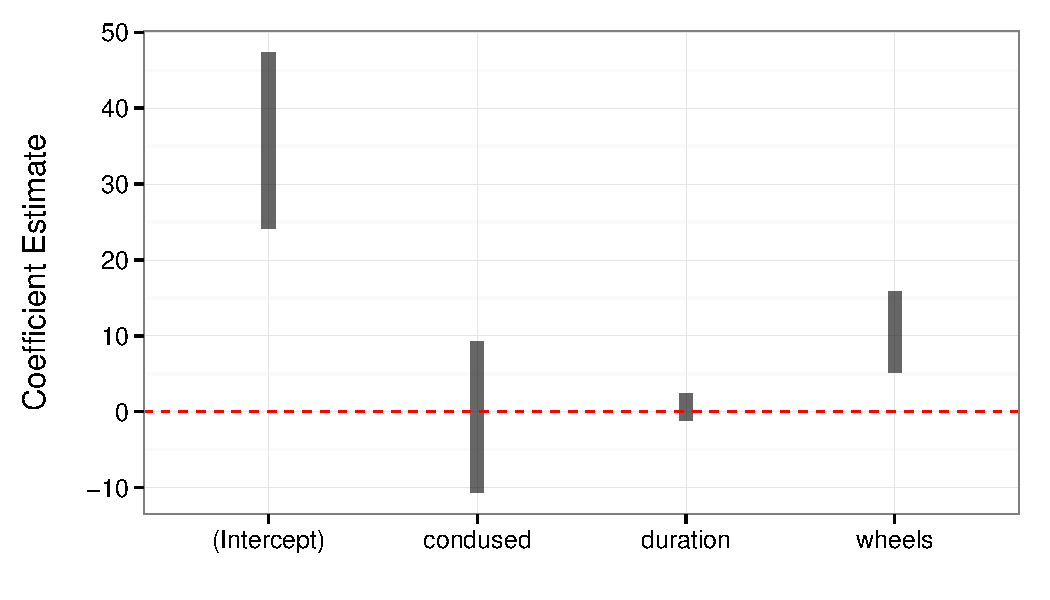
\includegraphics[width=\maxwidth]{figure/ConfIntGraph} 

}


\end{knitrout}

\end{frame}

%%%%% Model Assumptions
\section{Model Assumptions}
\frame{
  \frametitle{Multiple Linear Regression Model Assumptions}
  {\Large{Multiple Linear Regression Model Assumptions}}
  \begin{itemize}
    \item Nearly normally distributed residuals,
    \item Nearly constant residual variability,
    \item Residuals are independent,
    \item Each variable is linearly associated with the outcome
  \end{itemize}
}

%%% Model Selection (R2)
\section{Model Selection}
\frame{
  \frametitle{Model Selection with the Adjusted R Squared}
  \begin{center}
{\Large{How do we decide which variables to include in our multiple linear regression model?}}
  \end{center}
}

\frame{
  \frametitle{Omitted Variable Bias}
  We generally want to include all of the variables that have an important effect on the outcome. \\[0.5cm]
  Not including them creates \textbf{omitted variable bias}: i.e. our results are biased because we have omitted important variables.
}

\frame{
  \frametitle{However\ldots}
  We don't want to just include every variable we can think of into one model.
  \begin{itemize}
    \item \textbf{Occam's Razor: aim for parsimony (the simplest model possible).}
    \item The more variables you add, the {\bf{fewer degrees of freedom}} you will have to work with.
    \item You may include \textbf{highly correlated variables}, which can produce very biased estimates.
  \end{itemize}
}

\frame{
  \frametitle{The Adjusted $R^{2}$}
  We can use the \textbf{adjusted $R^{2}$} ($R^{2}_{adj}$)to determine if the addition of a variable to a linear regression model \textbf{reduces the errors} we make when predicting the outcome. 
  \[
  R^{2}_{adj} = \frac{Var(e_{i})/n - p - 1}{Var(y_{i})/(n - 1)}
  \]
  It is similar to the non-adjusted $R^{2}$ we learned about last week, but \textbf{only gets bigger if the addition of a variable reduces the errors} we make predicting the outcome.
}

\begin{frame}[fragile,plain]

\begin{table}[!ht]
\caption{Linear Regressions for Mario Kart Total Selling Price}
\label{} 
\begin{tabular}{ l D{.}{.}{2}D{.}{.}{2}D{.}{.}{2} } 
\hline 
  & \multicolumn{ 1 }{ c }{ Model 1 } & \multicolumn{ 1 }{ c }{ Model 2 } & \multicolumn{ 1 }{ c }{ Model 3 } \\ \hline
 %            & Model 1      & Model 2      & Model 3     \\ 
(Intercept)  & 38.41 ^{***} & 35.38 ^{***} & 35.73 ^{***}\\ 
             & (3.43)       & (5.27)       & (5.89)      \\ 
wheels       & 10.01 ^{***} & 10.58 ^{***} & 10.45 ^{***}\\ 
             & (2.41)       & (2.53)       & (2.70)      \\ 
duration     &              & 0.63         & 0.68        \\ 
             &              & (0.83)       & (0.91)      \\ 
condused     &              &              & -0.69       \\ 
             &              &              & (5.04)       \\
 $N$          & 143          & 143          & 143         \\ 
$R^2$        & 0.11         & 0.11         & 0.11        \\ 
adj. $R^2$   & 0.10         & 0.10         & 0.09        \\ 
Resid. sd    & 24.34        & 24.37        & 24.46        \\ \hline
 \multicolumn{4}{l}{\footnotesize{Standard errors in parentheses}}\\
\multicolumn{4}{l}{\footnotesize{$^\dagger$ significant at $p<.10$; $^* p<.05$; $^{**} p<.01$; $^{***} p<.001$}} 
\end{tabular} 
 \end{table}



\end{frame}

\frame{
  \frametitle{Model Section as Art}
  Model selection is something of an art, but it is useful to follow these \textbf{rules of thumb}:
  \begin{itemize}
    \item Drop highly insignificant variables, especially if they don't add to the adjusted $R^{2}$
    \item \textbf{Show a number of step-wise models} that could convince the reader that you have found the most {\bf{parsimonious}} model.
    \item Include results from \textbf{theoretically important} variables,
    \item \textbf{Avoid including highly correlated} variables in the same model,
    \item Don't show estimates from models that \textbf{violate linear regression assumptions},
  \end{itemize}
}

%%% Simulating expected values
\section{Simulating Expected Values}
\begin{frame}[fragile,plain]
  Though popular, tables like these are \textbf{not an effective way to communicate your findings}. \\[0.2cm]
  \begin{center}

 
\begin{tabular}{ l D{.}{.}{2}D{.}{.}{2}D{.}{.}{2} } 
\hline 
  & \multicolumn{ 1 }{ c }{ Model 1 } & \multicolumn{ 1 }{ c }{ Model 2 } & \multicolumn{ 1 }{ c }{ Model 3 } \\ \hline
 %            & Model 1      & Model 2      & Model 3     \\ 
(Intercept)  & 38.41 ^{***} & 35.38 ^{***} & 35.73 ^{***}\\ 
             & (3.43)       & (5.27)       & (5.89)      \\ 
wheels       & 10.01 ^{***} & 10.58 ^{***} & 10.45 ^{***}\\ 
             & (2.41)       & (2.53)       & (2.70)      \\ 
duration     &              & 0.63         & 0.68        \\ 
             &              & (0.83)       & (0.91)      \\ 
condused     &              &              & -0.69       \\ 
             &              &              & (5.04)       \\
 $N$          & 143          & 143          & 143         \\ 
$R^2$        & 0.11         & 0.11         & 0.11        \\ 
adj. $R^2$   & 0.10         & 0.10         & 0.09        \\ 
Resid. sd    & 24.34        & 24.37        & 24.46        \\ \hline
 \multicolumn{4}{l}{\footnotesize{Standard errors in parentheses}}\\
\multicolumn{4}{l}{\footnotesize{$^\dagger$ significant at $p<.10$; $^* p<.05$; $^{**} p<.01$; $^{***} p<.001$}} 
\end{tabular} 



  \end{center}
\end{frame}


\frame{
  \frametitle{Simulating Expected Values}
  Instead, King et al (2000) argue that we should find a way to \textbf{present results}, including our \textbf{estimation uncertainty} in relatively \textbf{simple language}.\\[0.5cm]
  They suggest that we simulated probable outcomes from our estimated models. \\[0.5cm]
  They (and others) created the \texttt{Zelig} package to help us simulate and graph expected outcomes.
}

\frame{
  \frametitle{\texttt{Zelig} Simulation Steps}
{\Large{\texttt{Zelig} Simulation Steps:}} \\[0.5cm]
  \begin{enumerate}
    \item Estimate model,
    \item Set fitted values,
    \item Simulate expected outcomes,
    \item Graph the simulated values.
  \end{enumerate}
}

\begin{frame}[fragile]
  \frametitle{\texttt{Zelig} Example}
  Simulated expected Total Mario Kart auction price with various numbers of included steering wheels.
\begin{knitrout}
\definecolor{shadecolor}{rgb}{0.969, 0.969, 0.969}\color{fgcolor}\begin{kframe}
\begin{alltt}
\hlcomment{# Load Zelig}
\hlfunctioncall{library}(Zelig)

\hlcomment{# Estimate model of total auction price with}
\hlcomment{# wheels and duration as independent variables}
ZOut <- \hlfunctioncall{zelig}(totalPr ~ wheels + duration,
              data = marioKart, model = \hlstring{"normal"},
              cite = FALSE)
\end{alltt}
\end{kframe}
\end{knitrout}

\end{frame}

\begin{frame}[fragile]
\begin{knitrout}
\definecolor{shadecolor}{rgb}{0.969, 0.969, 0.969}\color{fgcolor}\begin{kframe}
\begin{alltt}
\hlcomment{# Find valid range of wheels values}
\hlfunctioncall{range}(marioKart$wheels)
\end{alltt}
\begin{verbatim}
## [1] 0 4
\end{verbatim}
\begin{alltt}
\hlcomment{# Set fitted values for wheels}
\hlcomment{# Note: duration set at its mean}
WValues <- 1:4
XOut <- \hlfunctioncall{setx}(ZOut, wheels = WValues)

\hlcomment{# Simulate expected prices}
ZSim <- \hlfunctioncall{sim}(ZOut, x = XOut)
\end{alltt}
\end{kframe}
\end{knitrout}

\end{frame}

\begin{frame}[fragile]
\begin{knitrout}
\definecolor{shadecolor}{rgb}{0.969, 0.969, 0.969}\color{fgcolor}\begin{kframe}
\begin{alltt}
\hlcomment{# Plot middle 95% of the simulations}
\hlfunctioncall{plot}(ZSim, ylab = \hlstring{"Expected Price"}, 
     main = \hlstring{"Effect of Wheels on MK EBay Auctions"})
\end{alltt}
\end{kframe}

{\centering 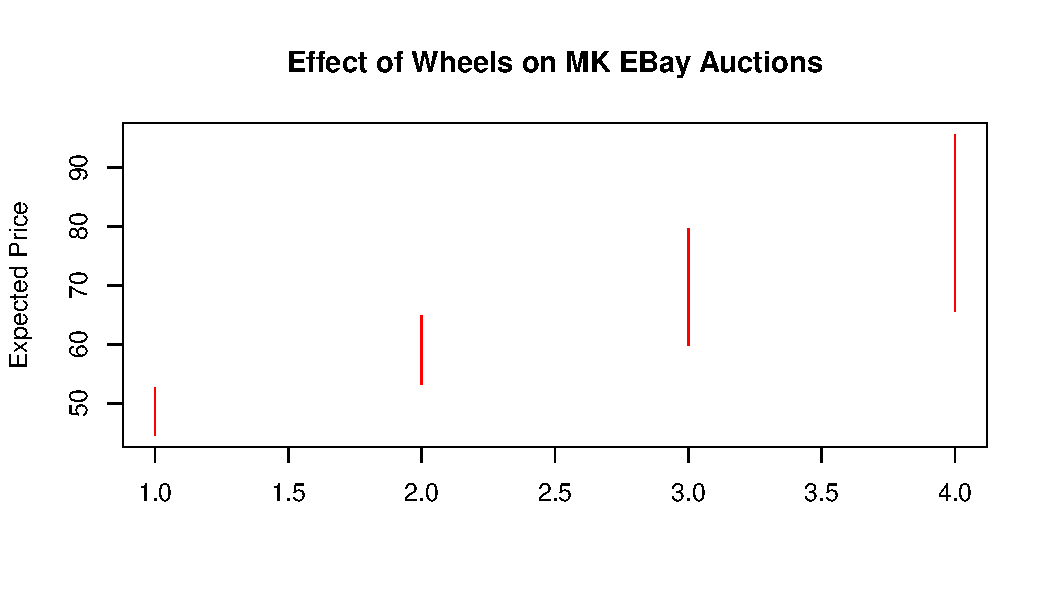
\includegraphics[width=\maxwidth]{figure/Zelig3} 

}


\end{knitrout}

\end{frame}

\frame{
  \frametitle{Question}
  \begin{center}
{\Large{Why is the predicted range of prices wider when there are 4 steering wheels?}}
  \end{center}
}

\frame{
  \frametitle{With (a lot) more work simulation graphs can look better}
  \begin{center}
    \includegraphics[scale=0.65]{/git_repositories/GreenBook/Paper/figure/ExpectValueParty.pdf}
  \end{center}
}
%%% References
\begin{frame}[allowframebreaks]
  \frametitle{References}
  Crawley, Michael J. 2005. Statistics: An Introduction Using R. Chichester: John Wiley & Sons. Ltd. \\[0.25cm]
  Diaz, David M., Christopher D. Barr, and Mine \c{C}etinkaya-Rundel. 2011. OpenIntro 
  Statistics. 1st ed. \url{http://www.openintro.org/stat/downloads.php}. \\[0.25cm] 
  King, Gary, Michael Tomz, and Jason Wittenberg. 2000. “Making the Most of Statistical Analyses: Improving Interpretation and Presentation.” American Journal of Political Science 44(2): 347–361.
\end{frame}

\end{document}
